\section{Gateway: Design \& Implementation}

\label{sec:gateway}
Having described our cryptographic building blocks, we can now discuss how they are used for encryption at the gateway.

\begin{figure}[t]
  \centering
  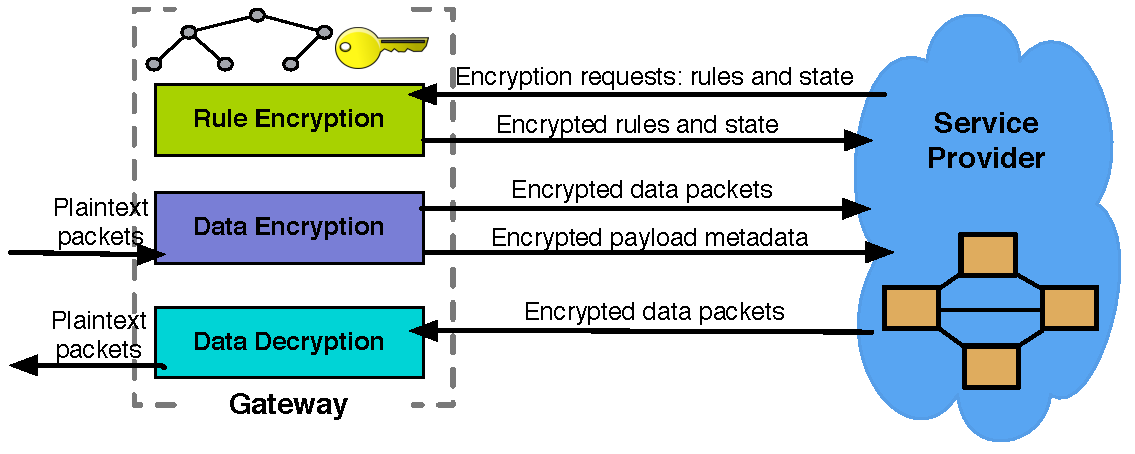
\includegraphics[width=3.25in]{fig/gateway2cloud}
  \caption[]{\label{fig:gatewaymeta} Communication between the cloud and gateway services: rule encryption, data encryption, and data decryption. \justine{Need to be consistent: is this a metadata channel or an extension channel}}
\end{figure}


\eat{
\begin{figure}[t]
  \centering
  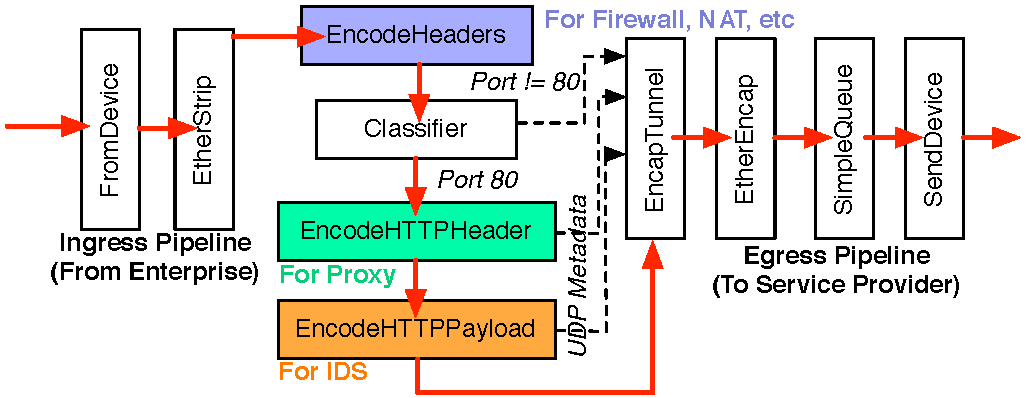
\includegraphics[width=3.25in]{fig/gatewaydiag}
  \caption[]{\label{fig:gateway} Data encryption (enterprise to cloud) click module.}
\end{figure}
}

The gateway serves two purposes. First, it redirects traffic to/from the cloud for middlebox processing. Second, it provides the cloud with encryptions of IDS/FW rulesets and updates to the RangeMatch tree.
Every gateway is configured statically to tunnel traffic to a fixed IP address at a single service provider point of presence.
A gateway can be logically thought of as three services: the rule encryption service, the pipeline from the enterprise to the cloud (Data encryption), and the pipeline from the cloud to the enterprise (Data decryption). 
All three services share access to the RangeMatch tree and the private key $k$.
Figure~\ref{fig:gatewaymeta} illustrates  these three services and the data they send to and from the cloud provider.

In what follows, we describe how the gateway performs rule encryption (\S\ref{sec:rulenc}), data encryption and decryption (\S\ref{sec:dataenc}), how the RangeMatch tree is managed and updated (\S\ref{sec:tree}), before discussing the gateways scalability, fault tolerance, and deployment requirements (\S\ref{sec:gwdiscuss}).
In \S\ref{sec:newmb} we return to the cloud and how middleboxes operate over the encrypted data there.

\subsection{Rule Encryption}
\label{sec:rulenc}


The rule encryption component provides the cloud provider with encrypted rules/policies to use at the middlebox. 
There are two possible ways rules can be generated. First, an enterprise may choose to generate their own rules, in which case, they send encrypted versions of the rules directly to the cloud.
Alternately, the enterprise may opt in to a `default' set of rules from the cloud provider, in which case the cloud provider sends the rules to the gateway which encrypts them and sends them back.
Rules can contain IP and transport header values -- which must be encrypted with RangeMatch -- or HTTP header fields, or DPI signatures, which must be encrypted with KeywordMatch.

The rule encryption component also handles rule updates. 
Whenever an adjustment is made to the RangeMatch table, it sends an update to the cloud provider with the adjusted mappings/rules.
If the gateway ever changes its key, the encryption component must also signal to the cloud provider and re-encrypt all rules.

\subsection{Data Encryption and Decryption}
\label{sec:dataenc}
\justine{Reiterate schemes.
Data dedup.
}
\subsection{The RangeMatch Tree}
\label{sec:tree}
Most encryption operations are relatively stateless -- they rely only on the key and the data. Using RangeMatch requires that the Rule Encryption component manage a tree of values for use at encryption time; we discuss how this tree is generated now.

The gateway keeps a small amount of state (in our implementation, about 200 bytes/range) encryption the intervals, but maintains no state per IP address encrypted or per connection. The gateway stores the tree in Fig.~\ref{fig:tree}: for each node, it stores the unencrypted endpoint, whether it is the left or  right margin of an interval, and the other endpoint of the interval it is part of. It does not need to store the encryption of the endpoint because this is easy to derive from the position in the tree. 


The gateway can use the following functions. EncryptRanges encrypts the initial ranges. Note that some ranges could consist of
one point only, namely $s = e$. 

% TO CUT TO REDUCE: put all these algorithms into one box
% framed takes space around it, above it, below it 

\begin{framed}
\begin{algorithmic}[1]

\Procedure{EncryptRanges}{[$s_1$, $e_1$], $\dots$, [$s_n$, $e_n$]}
  \State Build scapegoat tree on the values 
              $\{s_1, \dots, s_n\}$ 
              $\cup$ $\{e_1, \dots, e_n\}$ 
              $\cup$ $\{-\infty, \infty\}$.
  \State Assign an encryption $\enc(x)$ to each node $x$ in the tree:
  \begin{itemize}
  \item the root gets the middle of the IP range, $e$, 
  \item the node to the left of the root gets the middle of the interval to the left of $e$: ($e/2$),
  \item the right node gets the middle of the range
  to the right of $e$: ($3e/2$), and so on.
  \end{itemize}

  \State \Return{[$\enc(s_1)$, $\enc(e_1)$], $\dots$, [$\enc(s_n)$, $\enc(e_n)$]}
\EndProcedure

\end{algorithmic}
\end{framed}



EncryptValue encrypts the values to be matched against ranges.

\begin{framed}
\begin{algorithmic}[1]

\Procedure{EncryptValue}{$v$}
  \State Search the tree for $v$ to compute efficiently I as in Eq.~\ref{eq:randominterval}.
  \State Compute $\mathsf{index}(v) = \prf_k(v)\ \mod\ |I|.$ 
  \State Let $\enc(v)$ to be the $\mathsf{index}$-th element of $I$. 
  \State \Return $\left(\enc(v), \IV, \aes_k(\IV, v)\right)$ for random $\IV$. 
\EndProcedure

\end{algorithmic}
\end{framed}

Here is how to compute $I$ efficiently. When searching for $v$ in the tree, the gateway
can identify the tightest enclosing interval [$p_1$, $p_2$] in logarithmic time. 
 If $[p_1, p_2]$ are endpoints of the
same interval, then I = [$p_1$, $p_2$]. Otherwise, move towards the left in the tree until you identify the first endpoint
$\ell_1$
that belongs to an interval $[\ell_1, \ell_2]$ enclosing $v$. Then, using the tree, scan $[\ell_1, \ell_2]$ and eliminate
any intervals not containing $v$. The gateway can precompute and store this interval for every two consecutive nodes in the tree.

EncryptValue returns an AES encryption of $v$ too, because $\enc(v)$ is not decryptable. 

We now describe the procedure for AddRange and DeleteRange which add or delete an interval. 
These will modify the state at the gateway. Besides the interval added or deleted, a small number
of other intervals may be moved -- at worst, $O(\log n)$. For these, the algorithm returns the old and new encryption of the interval. 


\begin{framed}
\begin{algorithmic}[1]

\Procedure{AddRange}{$[s, e]$}
  \State Insert $s$ and $e$ into the scapegoat tree. If $s=e$, insert the value only once.
  %	
  \State Initialize $L$ to be the empty list.
  \If{tree needs to be rebalanced}
  	\State Record which nodes change position in the tree during rebalancing, together with 
	their old and new encryptions. Namely, record	\[L = \{ \en_1 \leftarrow \en^*_1, \dots, \en_m \rightarrow \en^*_m\},\] where $m$ is the number of nodes who changed position in the tree, and $\en_i$ and $\en^*_i$ are the old and new encryption of the $i$-th node that changed position. 
  \EndIf
  \State Compute  $\enc(s)$ and $\enc(e)$, the encryptions of $s$ and $e$, as in EncryptRanges.
   \State \Return{$[\enc(s), \enc(e)], L$}
\EndProcedure

\end{algorithmic}
\end{framed}

%  \State Determing the smallest and the largest encryption in the values $[\enc(s), \enc(e)]$ and $L$, and call this $\dirtyrange$.

Since we are using a scapegoat tree, the number of nodes that change position during rebalancing is amortized worst case $O(\log n)$ where $n$ is the total number of nodes in the scapegoat tree. 

DeleteRange is similar, except that the result contains only $L$. 

\eat{A natural question is whether there exists a scheme that does not need to adjust already encrypted intervals. For a related setting, Popa et al.~\cite{popa:mope} proved that whenever one supports ``>'' over  encrypted data, there must be some adjustment similar to this; the proof holds for our setting too.  }

\subsection{Discussion}
\label{sec:gwdiscuss}
\textbf{Scalability}
\textbf{Fault-Tolerance}
\textbf{Deployability}
